\documentclass{beamer}

%% \documentclass[handout]{beamer}
%% % use this with the [handout] option to create handouts for the audience
%% \usepackage{pgfpages}
%% \pgfpagesuselayout{2 on 1}[a4paper,border shrink=5mm]

\mode<presentation>
{
  \usetheme{Diku}
% set this to your preferences:
  \setbeamercovered{invisible}
%  \setbeamercovered{transparent}
}

\usepackage{graphicx}
\usepackage{epic}

\usepackage{amsmath}
\usepackage{amssymb}
\usepackage{amsthm}

\newcommand{\basetop}[1]{\vtop{\vskip-1ex\hbox{#1}}}
\newcommand{\source}[1]{\let\thefootnote\relax\footnotetext{\scriptsize\textcolor{kugray1}{Source: #1}}}

% for coloured code citation in text:
\usepackage{fancyvrb}

%%%%%%%%%%%%%%%%%%%%%%%%%%%%%%%%%
%%%%%    code sections   %%%%%%%%
%%%%%%%%%%%%%%%%%%%%%%%%%%%%%%%%%

% code highlighting commands in own block
\DefineVerbatimEnvironment{code}{Verbatim}{fontsize=\scriptsize}
\DefineVerbatimEnvironment{icode}{Verbatim}{fontsize=\scriptsize}

% Fancy code with color commands:
\DefineVerbatimEnvironment{colorcode}%
        {Verbatim}{fontsize=\scriptsize,commandchars=\\\{\}}

%%%%%%%%%%%%%%%%%%%%%%%%%%%%%%%%%%
%%%%%    some coloring    %%%%%%%%

\definecolor{Red}{RGB}{220,50,10}
\definecolor{Blue}{RGB}{0,51,102}
\definecolor{Yellow}{RGB}{102,51,0}
\definecolor{Orange}{RGB}{178,36,36}
\definecolor{Grey}{RGB}{180,180,180}
\definecolor{Green}{RGB}{20,120,20}
\definecolor{Purple}{RGB}{160,50,100}
\newcommand{\red}[1]{\textcolor{Red}{{#1}}}
\newcommand{\blue}[1]{\textcolor{Blue}{{#1}}}
\newcommand{\yellow}[1]{\textcolor{Yellow}{{#1}}}
\newcommand{\orange}[1]{\textcolor{Orange}{{#1}}}
\newcommand{\grey}[1]{\textcolor{Grey}{{#1}}}
\newcommand{\green}[1]{\textcolor{Green}{{#1}}}
\newcommand{\purple}[1]{\textcolor{Purple}{{#1}}}




% use "DIKU green" from our color theme for \emph
\renewcommand{\emph}[1]{\textcolor{structure}{#1}}
% use some not-too-bright red for an \emp command
\definecolor{DikuRed}{RGB}{130,50,32}
\newcommand{\emp}[1]{\textcolor{DikuRed}{ #1}}
\definecolor{CosGreen}{RGB}{10,100,70}
\newcommand{\emphh}[1]{\textcolor{CosGreen}{ #1}}
\definecolor{CosBlue}{RGB}{55,111,122}
\newcommand{\emphb}[1]{\textcolor{CosBlue}{ #1}}
\definecolor{CosRed}{RGB}{253,1,1}
\newcommand{\empr}[1]{\textcolor{CosRed}{ #1}}

\newcommand{\mymath}[1]{$ #1 $}
\newcommand{\myindx}[1]{_{#1}}
\newcommand{\myindu}[1]{^{#1}}

\newcommand{\Fasto}{\textsc{Fasto}\xspace}


%%%%%%%%%%%%%%%%%%%%

\title[S-TLS]{Software Thread-Level Speculation (S-TLS)}

\author[C.~Oancea]{Cosmin E. Oancea\\{\tt cosmin.oancea@diku.dk}}

\institute{Department of Computer Science (DIKU)\\University of Copenhagen}


\date[Oct'14]{October 2014 PMPH Lecture Notes}


\begin{document}

\titleslide

\begin{frame}
\frametitle{Course Organization}

\begin{tabular}{lccccc}
W  & HARDWARE  & & SOFTWARE     & & LAB/CUDA \\\hline\hline
1 & Trends        &                         & List HOM     & & Intro \& Simple\\
  & Vector Machine & $\longleftarrow$ & (Map-Reduce) & & Map Programming\\\hline
%
2 & In Order & $\longrightarrow$ & VLIW Instr   & & Scan \&\\
  & Processor& $\longleftarrow$ & Scheduling   & & Reduce \\\hline
%
3 & \emphh{Cache}     & & Reasoning About     & & Sparse Vect\\
  & \emphh{Coherence} & & Parallelism   & & Matrix Mult\\\hline
%
4 & Interconnection & & Case Studies \&   & & Transpose \& Matrix\\
  & Networks        & & Optimizations   & & Matrix Mult\\\hline
%
5 & \emphh{Memory}      & & Optimising   & & Sorting \& Profiling \& \\
  & \emphh{Consistency} & & Locality     & & Mem Optimizations \\\hline
%
6 & \emphh{OoO, Spec}   & $\longleftarrow$ & \alert{Thread-Level}   & & Project \\
  & \emphh{Processor}   & & \alert{Speculation}    & & Work    \\\hline

%\framebox{Processor}       & & \framebox{Low-Level\\Optimizations}        & & \framebox{CUDA: Scan\\Reduce}\\
%$\downarrow$ && $\uparrow$ \\
%\framebox{\red Intermediate code generation} &$\longrightarrow$ & Intermediate code
\end{tabular}
\medskip
%\alert{Keywords: Reasoning, Tradeoffs, Common Case, }

Three narative threads: the path to complex \& good design: 
\begin{itemize}
    \item \emp{Design Space} tradeoffs, constraints, common case, trends.
    \item \emp{Reasoning}: from simple to complex, \emp{Applying Concepts}.
\end  {itemize}
\end{frame}



%%%%%%%% real content starts here %%%%%%%%%%

\begin{frame}[fragile]
	\tableofcontents
\end{frame}

\section{Motivation for Thread-Level Speculation (TLS)}

\begin{frame}[fragile,t]
  \frametitle{Motivation for Thread-Level Speculation (TLS)}

Consider a sequential program in a mainstream language (C{\tt ++}, Java).

\emp{Automatic parallelization may fail due to:}
\begin{itemize}
    \item indirect arrays, or pointers (aliasing), or
    \item loops with false dependencies,
    \item large loops with complex indexing and control flow,
    \item partially-parallel loops, 
            i.e., occasional cross-iter dependency.
\end  {itemize}\medskip

\begin{block}{Simplified Fast Fourier {\tt~~~~~~~} and Floyd Warshall}
\begin{columns}
\column{0.47\textwidth}
\begin{colorcode}
for(dual=1; dual<n; dual*=2) // \emp{seq}
  for(a=0; a<dual; a++) // \emphh{parallel}
    for(b=0; b<n; b+=2*dual)      \{ 
      int i=2*(b+a), j=2*(b+a+dual); 
      X[j] = Exp(X[j+1], X[j]);  
      X[i] = Exp(X[i+1], X[i]); ... 
    \} 
\end{colorcode}
\column{0.47\textwidth}
\begin{colorcode}
for(k=0; k<N; k++) \{  // \emp{seq}
  for(i=0; i<N; i++) \{// \emphh{parallel?}
    for(j=0; j<N; j++) \{
      \purple{X[i,j]} = X[i,k] + \purple{X[k,j]};
    \}
  \}
\}
\end{colorcode}
\end{columns}
%\column{0.47\textwidth}
%\begin{colorcode}
%// \blue{X}: indirect array of size N,
%//   with elems \mymath{\in} \{0..N-1\}
%// \blue{mat}: a NxM matrix, with M >= 32. 
%for(int i=0; i < N; i++)\{//\emphh{parallel?}
%  float* row = &mat[ X[i]*M ];
%  for(int j=1; j < M; j++) \{ //\emp{seq}
%    row[j] = sqrt(row[j-1]+row[j]);
%\} \}
%\end{colorcode}
\end{block} 

\emp{Both loops have (simple) affine indices. Still, the LEFT one
is difficult to prove parallel, the other has 
dependencies involving iteration {\tt i=k}.}

\end{frame}


\begin{frame}[fragile,t]
  \frametitle{Motivation for Thread-Level Speculation (TLS)}

\begin{block}{Loops with Indirect Arrays Cannot Be Parallelized Statically!}
\begin{columns}
\column{0.47\textwidth}
\begin{colorcode}
// \blue{A} array of size M
// \blue{X and Y} indirect arrays
//   of size N with elements
//   in \{0...M-1\} 
for(i=0; i<N; i++) \} // \emphh{parallel?}
    A[X[i]] = ... A[Y[i]] ...
\}
\end{colorcode}
\begin{scriptsize}
\begin{itemize}
\item If X = Y = \{0...N-1\}\\\pause
        then the loop is parallel.
\item If X = \{0, 2,...\} and Y = \{1, 0,...\}
        then\pause {\tt~}cross
        iteration dependency between iterations
        {\tt 0} and {\tt 1}. 
\end{itemize}
\end{scriptsize}
\column{0.50\textwidth}
\begin{colorcode}
// \blue{X}: indirect array of size N,
//   with elems \mymath{\in} \{0..N-1\}
// \blue{mat}: a NxM matrix. 
for(int i=0; i < N; i++)\{//\emphh{parallel?}
  float* row = &mat[ X[i]*M ];
  for(int j=1; j < M; j++) \{ //\emp{seq}
    row[j] = sqrt(row[j-1]+row[j]);
\} \}
\end{colorcode}
\begin{scriptsize}
\begin{itemize}
\item If X is a permutation of \{0...N-1\}\\\pause
        then the loop is parallel.
\item If X is not a permutation then there
        are cross iteration dependencies!
\end{itemize}
\end{scriptsize}
\end{columns}
\end{block} 

Both loops may or may not be parallel due to indirect
arrays ... but we can \alert{speculate} that they are 
(due to the huge benefit of paralleliz.)
\medskip

\emphh{TLS is an universal panacea of parallelization:
speculate that loop is parallel \& devise a mechanism
to track and recover from violations!}

\end{frame}

\section{S-TLS Execution Model}

\begin{frame}[fragile]
	\tableofcontents[currentsection]
\end{frame}


\begin{frame}[fragile,t]
  \frametitle{High-Level TLS Design}

\begin{itemize}
\item Rauchwerger and Padua. ``{\em The LRPD Test: Speculative Run-Time 
        Parallelization of Loops with Privatization and 
        Reduction Parallelization}'', 
        IEEE TPDS, 10 No 2(2), Feb 1999.\medskip

\item TLS: entirely dynamic parallelization technique that executes
        loop iterations out of order, even in the
        presence of cross iteration dependencies, \blue{which are tracked
        and fixed at runtime}.\medskip

\item \blue{TLS typically isolate the speculative state from the global state:}\\
        each thread buffers its updates, and \emp{commits} them only when 
        speculation up-to-that thread is \emp{guaranteed} to have succeeded.

\item \emphh{Follows that {\sc waw} and {\sc war} dependencies are 
                implicitly enforced.}
        \emp{Whaaattt does ``guaranteed'' mean? When does commit happen?}\medskip\pause

\item The thread executing the lowest-numbered iteration is called \emphh{\sc master}:
        it encapsulates both the correct state and control flow.\medskip

\item At the end of its iteration, the thread waits to become {\sc master}
        and then commits $\Rightarrow$ progress is guaranteed.
\end{itemize}

\end{frame}


\begin{frame}[fragile,t]
  \frametitle{Ideal Execution (No Violations)}

\begin{columns}
\column{0.35\textwidth}
%\vspace{-15ex}
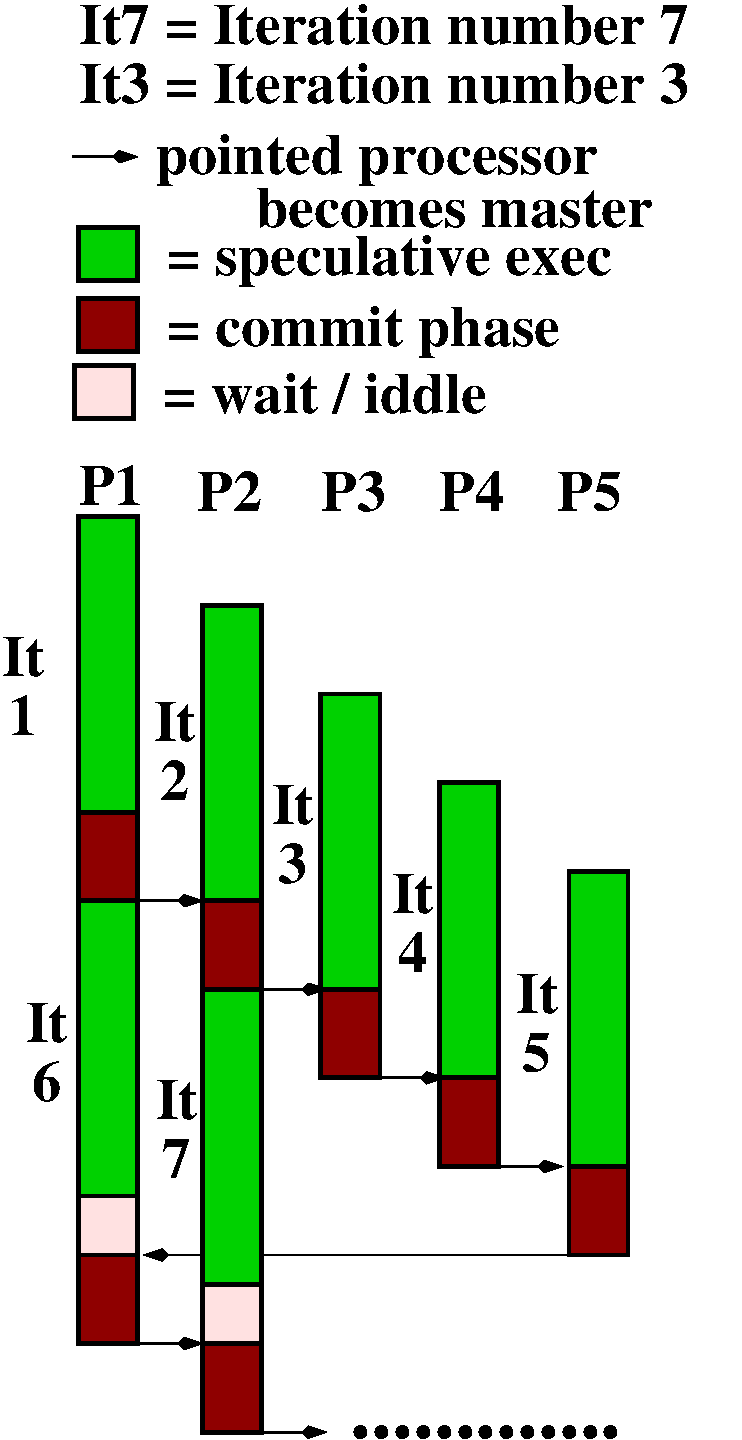
\includegraphics[width=22ex]{FigsTLS/IdealCommit.pdf}\pause
\column{0.62\textwidth}
%\begin{scriptsize}
\begin{itemize}
\item Note that the commit phase is serial!
\item Amdhal's law is unforgiving: even under 
        NO violations, the number of processors 
        that contribute
        to speedup is limited by the weight
        of the commit phase, i.e., \#
        of per-iter updates.\medskip

\item \emp{How to track dependency violations?}
\item Uses vectors to record which thread has
        read/written each mem location.
\item Extended cache-coherence protocol for
        dependency tracking and rollback.
\item Hardware TLS: more efficient than software, BUT
        limited speculative storage may restrict the ability
        to exploit coarser levels of parallelism. 
\end{itemize}
%\end{scriptsize}
\end{columns}

\end{frame}


\begin{frame}[fragile,t]
  \frametitle{Speculative Execution with Rollbacks}

\begin{columns}
\column{0.70\textwidth}
%\vspace{-15ex}
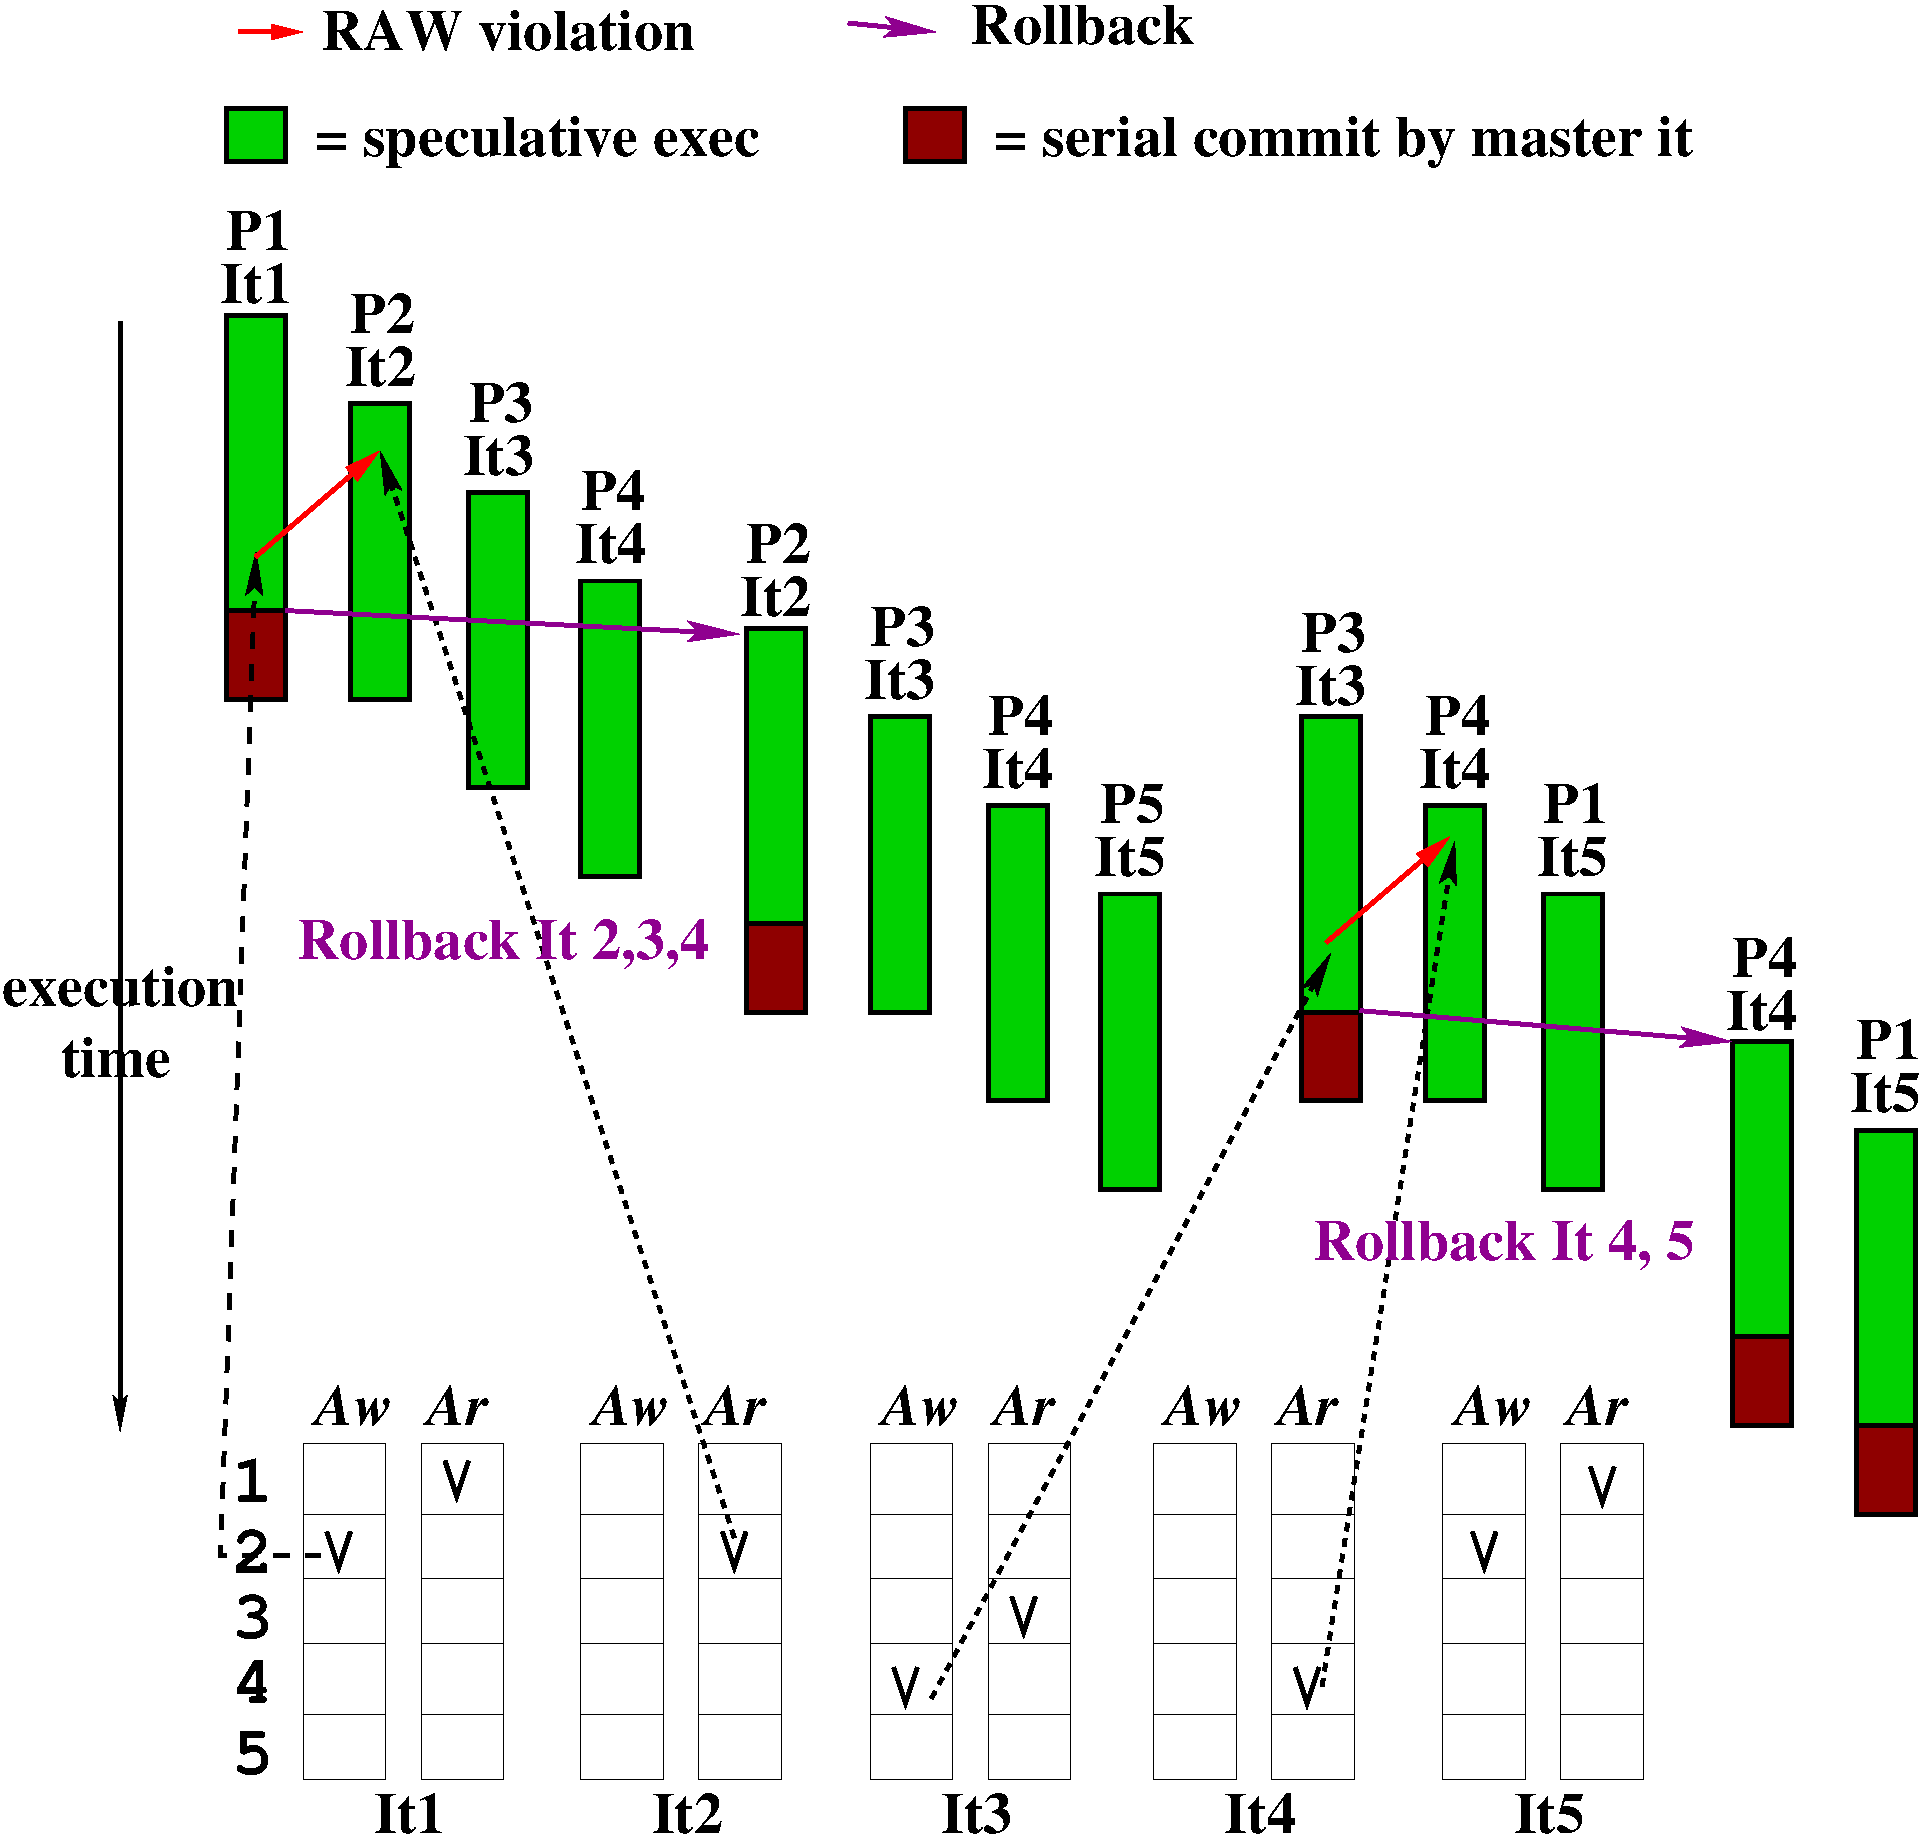
\includegraphics[width=47ex]{FigsTLS/Rollback.pdf}\pause
\column{0.42\textwidth}
\begin{scriptsize}
\begin{itemize}
\item \emp{How to track dependency violations?}
\item Load/Store vectors, which are maintained per mem location
        and per iteration (processor), are used to track 
        dependencies.
\item Normal load/store operations are replaced with 
        function calls that use the Load/Store vectors 
        and simulate a cache coherence protocol.
\item If a violation is encountered, then the thread
        waits to become master, commits, stops all other threads,
        and execute a \emp{rollback procedure} to bring
        execution to a safe point.
\item Rollback simply discards the speculative storage,
        clears the Load/Store vectors, and restarts
        speculative exec. 
\end{itemize}
\end{scriptsize}
\end{columns}

\end{frame}

\section{S-TLS Naive Dependency Tracking Implementation}

\begin{frame}[fragile]
	\tableofcontents[currentsection]
\end{frame}

\begin{frame}[fragile,t]
  \frametitle{A Very Simplified Dependence Tracking Implem}

Rundberg and Stenstrom. ``{\em An All-Software Thread-Level Data Dependence Speculation System for Multiprocessors.}'', Journal of Instruction-Level Parallelism, 1999.\medskip

\begin{columns}
\column{0.5\textwidth}
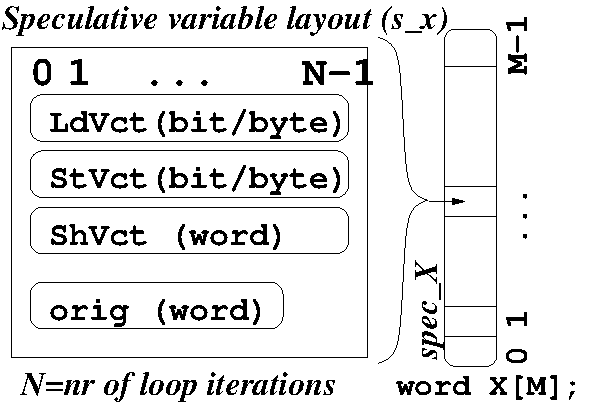
\includegraphics[width=28ex]{FigsTLS/SpecMemSeminal.pdf}
\column{0.47\textwidth}\vspace{-2ex}
\begin{colorcode}
\emp{DO} i = 1, N
  \emp{X(A(i))} = ... \emp{X(B(i))} ...
ENDDO

\mymath{\downarrow \ \downarrow \ \downarrow}
\emphh{DOALL} i = 1, N
  val = spec_X.\emphh{specLD(B(i), i)}
  spec_X.\emphh{specST(A(i), ... val ..., i)}
  IF is_rollback() THEN rollback()
ENDDO
\end{colorcode}
\end{columns}
\medskip\pause

\begin{columns}
\column{0.44\textwidth}
\begin{colorcode}
\emphh{WORD specLD(int ind, int itNr)} \{
  \blue{LdVct[ind][itNr] = 1;}

  \emp{int i = highest index marked}
          \emp{in StVct[ind] <= itNr;}
  if(i>=0) return ShVct[ind][i];
  else return orig;
\}
\end{colorcode}
\column{0.53\textwidth}
\begin{colorcode}
\emphh{void specST( int ind, WORD val, int itNr )} \{  
  ShVct[ind][itNr] = val;            
  \blue{StVct[ind][itNr]  = 1;}
  
  if( \emp{exists i > itNr with} 
         \emp{LdVct[ind][i]==1} )
    \alert{Mark_Dep_Exc(i);}
\}
\end{colorcode}
\end{columns}

\end{frame}

\begin{frame}[fragile,t]
  \frametitle{Similarities With OoO Processor \& Coherence}

\begin{itemize}
\item Serial commit phase $\Leftrightarrow$ reorder buffer (ROB).\medskip
\item Speculative storage $\Leftrightarrow$ renaming registers in ROB +
        speculative state between the end of execution and commit at top of ROB.\medskip
\item In both cases this solves {\sc war} and {\sc waw} dependencies.\medskip
\item The use of speculative state {\tt ShVct} $\Leftrightarrow$ forwarding 
        values between various pipeline stages.\medskip
\item Rollback discards speculative state $\Leftrightarrow$ rollback 
        discards all instructions in ROB and back end and resumes
        fetching.\bigskip

\item The use of load/store vectors {\tt LdVect/StVct} $\Leftrightarrow$
        resembles a cache coherence protocol.
\end{itemize}

\end{frame}

\begin{frame}[fragile,t]
  \frametitle{A Very Simplified Dependence Tracking Implem}

\alert{Why is the implementation on the previous slide naive?}\smallskip\pause

\begin{itemize}
\item Original memory is $O(M)$. Speculative memory: $O(M\times N)$ ???\medskip
\item Original read/write is $O(1)$. {\tt SpecLD}/{\tt SpecST} is $O(N)$ ???
\end{itemize}\bigskip

\purple{How to improve it?}\smallskip\pause
\begin{itemize}
\item If we guarantee that only {\tt P} iterations can run concurrently 
        at any time then we can size {\tt LdVct}/{\tt StVct}/{\tt ShVct} 
        to {\tt P} words.\medskip
\item It follows speculative memory $O(M\times P)$ and {\tt specLD/ST} $O(P)$.\medskip
\item The asymptotic is still wrong: we use {\tt P} processors but work is $O(P*N)$
        instead of $O(N)$.\medskip
\item Gives speedup if relatively few instructions need to be protected
        with TLS support, i.e., most of them disambiguated statically.\medskip
\item Other special tricks to optimize the common case, e.g., hold one field
        the entry in {\tt LdVct} ({\tt StVct}) recording whether any iteration
        has accessed the element. If not then {\tt SpecLD}/{\tt SpecST} are $O(1)$.
\end{itemize} 

\end{frame}


\begin{frame}[fragile,t]
  \frametitle{Is Algorithm Race Free \& Respects Memory Model?}

\begin{itemize}
\item \emp{Does it need locking}, i.e., do {\tt specLD/ST} need to execute atomically?\pause
        \emphh{No, it is safe as it is (resembles Decker's alg).}\medskip

\item \emp{Any troubles with memory consistency?}\pause\\
    \alert{Yes}, most/all hardware use store-load relaxation, and this
        access pattern appears between \alert{{\tt LdVct} and {\tt ShVct}}!\medskip

\item Store-load relaxation requires memory fences, which are expensive.
        \alert{Is there a cheaper way?}\pause\medskip
\begin{itemize}
    \item memory model refers to reordering between 2 different locations
    \item if we interleave the same entry of {\tt LdVct}, {\tt StVct}
            and {\tt ShVct} into the same word (memory block) then
            we have turned it into a cache coherency problem $\Rightarrow$
            no need for memory fences! 
\end{itemize}
\end{itemize}\bigskip

Note that we have not entered all details. For example in order to commit
efficiently, each thread needs to keen track of what it has modified.
In addition it should also clear its {\tt Ld/StVect} entries.

\end{frame}


\section{A Family of Lightweight S-TLS Implementations}

\begin{frame}[fragile]
	\tableofcontents[currentsection]
\end{frame}

\begin{frame}[fragile,t]
  \frametitle{Lightweight S-TLS Tradeoff}

Oancea, Mycroft and Harris. 
``{\em A Lightweight In-Place Implementation for 
Software Thread-Level Speculation''}, SPAA'09.\medskip

{\bf Tutorial and library code \& benchmark available as:\\
http://www.diku.dk/$\sim$zgh600/tlsindex.html}\medskip

\bigskip

Goals:
\begin{itemize}
    \item[+] \emphh{Serial commit phase does not scale with the 
                \# of processors $\Rightarrow$ would like an ``in-place'' 
                update implementation.}\medskip
    \item[+] \emphh{Would like to have a speculative memory of size less than the
            original array (and ideally negligible) 
            INSTEAD of {\tt P} times the size of the array.}\medskip
    \item[+] \emphh{Would like to have $O(1)$ {\tt specLD/ST} instead of $O(P)$.}\medskip
    \item[-] \emp{We are willing to pay with the occasional 
                false-positive violation, i.e., few number of rollbacks
                that may not be necessary,} 
    \item[-] \emp{also in-place update means {\sc war} and {\sc waw} are NOT enforced}.
\end{itemize}

\end{frame}


\begin{frame}[fragile,t]
  \frametitle{Lightweight S-TLS Dependency Tracking}

\begin{columns}
\column{0.5\textwidth}
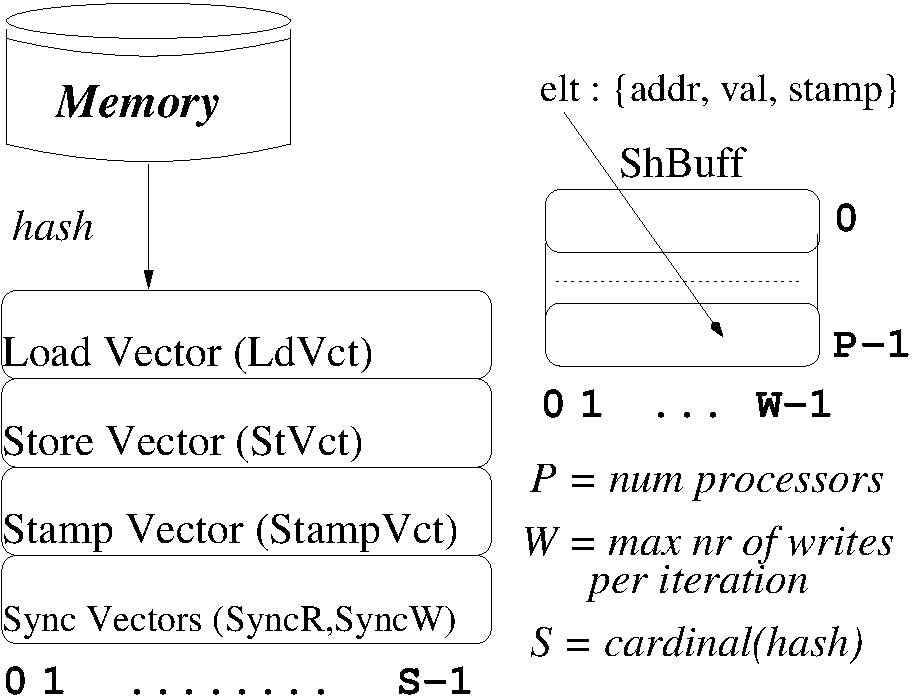
\includegraphics[width=28ex]{FigsTLS/SpecMem1.pdf}
\column{0.47\textwidth}\vspace{-2ex}
\begin{colorcode}
\emp{DO} i = 1, N
  \emp{X(A(i))} = ... \emp{X(B(i))} ...
ENDDO

\mymath{\downarrow \ \downarrow \ \downarrow}
\emphh{DOALL} i = 1, N
  val = spec_X.\emphh{specLD(B(i), i)}
  spec_X.\emphh{specST(A(i), ... val ..., i)}
  IF is_rollback() THEN rollback()
ENDDO
\end{colorcode}
\end{columns}
\medskip\pause

\begin{itemize}
    \item Let {\tt hash : $\mathbb{Z} \rightarrow \{0,\ldots,S-1\}$},
            where {\tt hash} and $S$ are found via dynamic analysis (profiling).
    \item The size {\tt LdVct}, {\tt StVct}, etc., is $S$ words 
            ($\times$ cache line size).
    \item \emp{StampVct} holds the ``current time'' of an update,
    \item \emp{\bf Each thread updates global memory in-place, but it stores the
            prior-held value in thread private storage {\tt ShBuff}}. 
    \item An access to location {\tt a} is treated as if all 
            memory locations in {\tt a}'s equiv class were accessed, 
            i.e., {\tt$\forall$b s.th. hash(a)=hash(b)}: 
%    \item {\tt Ld/StVct[i]} holds the highest iteration (number) that
%            has read/written any memory location {\tt a} such that {\tt hash(a) = i}.
\end{itemize}

\end{frame}


\begin{frame}[fragile,t]
  \frametitle{First Implementation: Lightweight S-TLS}

\begin{columns}
\column{0.32\textwidth}
\begin{colorcode}
\emp{atomic} WORD \emphh{specLD}(volatile
      WORD* addr, int itNr)\{
1   int i = hash(addr);
2   \emphh{if(LdVct[i]<thNr)}
3      \emphh{LdVct[i]=itNr;}
4   WORD val = *addr;
5   if(StVct[i]<=itNr)
6      return val;
7   \emp{else throw}
8     \emp{Dep_Exc(itNr-1);}    \}
\end{colorcode}
\column{0.55\textwidth}
\begin{colorcode}
\emp{atomic} void \emphh{specST}( volatile WORD* addr,
                    WORD new_val, int itNr) \{
1   int i    = hash(addr);
2   int prev = StVct[i];
3   \purple{if(prev > itNr) throw Dep_Exc(itNr-1);}
5   \emphh{StVct[i] = itNr;}
6   \blue{save( addr, *addr, StampVct[i]++ );}
7   *addr     = new_val;
8   WORD load = LdVct[i];
9   \alert{if(load > itNr) throw Dep_Ex(itNr-1);}  \}
\end{colorcode}
\end{columns}
\medskip\pause

\begin{itemize}
    \item {\tt specST/specLD} execute atomically (expensive). No forwarding.
    \item \emphh{{\tt Ld/StVct[i]} holds the highest iteration (number) that
            has read/written any memory location {\tt a} such that {\tt hash(a) = i}.}
    \item \emp{If {\tt StVct[i]>itNr} then a successor iteration has written the
                value in global memory $\Rightarrow$ {\sc war} violation}!
    \item \purple{If {\tt StVct[i]>itNr} then the current thread needs to overwrite
                a successor iteration $\Rightarrow$ {\sc waw} violation}!
    \item \alert{If {\tt LdVct[i]>itNr} then a successor iter has consumed
                another value than the one produced by the current iter $\Rightarrow$ {\sc raw} violation.}
\end{itemize}

\end{frame}


\begin{frame}[fragile,t]
  \frametitle{First Implementation: Lightweight S-TLS}

\begin{columns}
\column{0.32\textwidth}
\begin{colorcode}
\emp{atomic} WORD \emphh{specLD}(volatile
      WORD* addr, int itNr)\{
1   int i = hash(addr);
2   \emphh{if(LdVct[i]<thNr)}
3      \emphh{LdVct[i]=itNr;}
4   WORD val = *addr;
5   if(StVct[i]<=itNr)
6      return val;
7   \emp{else throw}
8     \emp{Dep_Exc(itNr-1);}    \}
\end{colorcode}
\column{0.55\textwidth}
\begin{colorcode}
\emp{atomic} void \emphh{specST}( volatile WORD* addr,
                    WORD new_val, int itNr) \{
1   int i    = hash(addr);
2   int prev = StVct[i];
3   \purple{if(prev > itNr) throw Dep_Exc(itNr-1);}
5   \emphh{StVct[i] = itNr;}
6   \blue{save( addr, *addr, StampVct[i]++ );}
7   *addr     = new_val;
8   WORD load = LdVct[i];
9   \alert{if(load > itNr) throw Dep_Ex(itNr-1);}  \}
\end{colorcode}
\end{columns}
\medskip\pause

\begin{itemize}
    \item {\tt specST/specLD} execute atomically (expensive). No forwarding.\medskip
    \item \blue{Before updating the global memory, the global-memory value is
                saved in {\tt ShVct} together with the time stamp of the update
                ({\tt StampVct[i]} holds the current time).}\medskip
    \item In case of violation, the global memory can be rolled back to 
            the correct one with the information in {\tt ShVct}.\medskip

    \item Note that the rollback is more complex/expensive than with the serial commit.
\end{itemize}

\end{frame}

\begin{frame}[fragile,t]
  \frametitle{Second Implem: Lock-Free Lightweight S-TLS}

\begin{columns}
\column{0.32\textwidth}
\begin{colorcode}
WORD specLD( volatile WORD* 
addr, int itNr, int TH_ID ) \{ 
1 int i = hash(addr); 
2 \purple{SyncW[i] = TH_ID;} 
3 
4 if( LdVct[i] < itNr )
5     LdVct[i] = itNr; 
6 
7 if( \purple{SyncW[i] != TH_ID} ) 
8   \emp{SyncR[i] = itNr + P;} 
9 
10 WORD val = *addr; 
11 if( StVct[i] <= itNr ) 
12      return val;
13 else throw Dep_Exc(itNr-1);
\} 
\end{colorcode}
\column{0.55\textwidth}
\begin{colorcode}
void specST( volatile WORD* addr,
            WORD new_val, int itNr, int TH_ID)\{
1  int i = hash(addr);
2  \purple{SyncW[i] = TH_ID;}
3
4  if(StVct[i] > itNr) throw Dep_Exc( itNr-1 );
5  StVct[i] = itNr;
6
7  if(\purple{SyncW[i] != TH_ID}) \alert{throw Dep_Exc( itNr-1 );}
8  save( addr, *addr, StampVct[i]++ );
10 *addr = new_val;
11
12 WORD ld = \emp{max( LdVct[i], \emp{SyncR[i]} );}
13 if( (\alert{ld > itNr}) || (StVct[i] != itNr) )
14 throw Dep_Exc( itNr-1 ); 
\}
\end{colorcode}
\end{columns}
\medskip\pause

\begin{itemize}
    \item \emp{\tt specST--specLD} interaction was safe as it previously was.\medskip
    \item \emp{\tt specLD--specLD} and \emp{specST--specST} interactions exhibit
            race conditions: these are very rare $\Rightarrow$ CHEAPER to solve by 
            raising the occasional false-positive rollback THAN by locking!
\end{itemize}
\end{frame}

\begin{frame}[fragile,t]
  \frametitle{Second Implem: Lock-Free Lightweight S-TLS}

\begin{columns}
\column{0.32\textwidth}
\begin{colorcode}
WORD specLD( volatile WORD* 
addr, int itNr, int TH_ID ) \{ 
1 int i = hash(addr); 
2 \purple{SyncW[i] = TH_ID;} 
3 
4 if( LdVct[i] < itNr )
5     LdVct[i] = itNr; 
6 
7 if( \purple{SyncW[i] != TH_ID} ) 
8   \emp{SyncR[i] = itNr + P;} 
9 
10 WORD val = *addr; 
11 if( StVct[i] <= itNr ) 
12      return val;
13 else throw Dep_Exc(itNr-1);
\} 
\end{colorcode}
\column{0.55\textwidth}
\begin{colorcode}
void specST( volatile WORD* addr,
            WORD new_val, int itNr, int TH_ID)\{
1  int i = hash(addr);
2  \purple{SyncW[i] = TH_ID;}
3
4  if(StVct[i] > itNr) throw Dep_Exc( itNr-1 );
5  StVct[i] = itNr;
6
7  if(\purple{SyncW[i] != TH_ID}) \alert{throw Dep_Exc( itNr-1 );}
8  save( addr, *addr, StampVct[i]++ );
10 *addr = new_val;
11
12 WORD ld = \emp{max( LdVct[i], \emp{SyncR[i]} );}
13 if( (\alert{ld > itNr}) || (StVct[i] != itNr) )
14 throw Dep_Exc( itNr-1 ); 
\}
\end{colorcode}
\end{columns}
\medskip\pause

For example, take \emp{\tt specLD--specLD} races:
        \begin{itemize}
            \item \purple{{\tt SyncW[i]} verifies that there was no race condition 
                    on {\tt LdVct[i]}}
            \item \emp{IF race occurs, we do not yet raise a violation,
                    but conservatively set {\tt SyncR[i]} to an iter \#
                    higher than any who are currently executed $\Rightarrow$ the false
                    positive might be raised in {\tt specST}}. 
        \end{itemize}
\end{frame}

\begin{frame}[fragile,t]
  \frametitle{Third Implem: Lightweight S-TLS Free of Fences}

\begin{columns}
\column{0.32\textwidth}
\begin{colorcode}
WORD specLD( volatile WORD* 
addr, int itNr, int TH_ID ) \{ 
1 int i = hash(addr); 
2 \purple{SyncW[i] = TH_ID;} 
3 
4 if( LdVct[i] < itNr )
5     LdVct[i] = itNr; 
6 
7 if( \purple{SyncW[i] != TH_ID} ) 
8   \emp{SyncR[i] = itNr + P;} 
9 
10 WORD val = *addr; 
11 if( StVct[i] <= itNr ) 
12      return val;
13 else throw Dep_Exc(itNr-1);
\} 
\end{colorcode}
\column{0.55\textwidth}
\begin{colorcode}
void specST( volatile WORD* addr,
            WORD new_val, int itNr, int TH_ID)\{
1  int i = hash(addr);
2  \purple{SyncW[i] = TH_ID;}
3
4  if(StVct[i] > itNr) throw Dep_Exc( itNr-1 );
5  StVct[i] = itNr;
6
7  if(\purple{SyncW[i] != TH_ID}) \alert{throw Dep_Exc( itNr-1 );}
8  save( addr, *addr, StampVct[i]++ );
10 *addr = new_val;
11
12 WORD ld = \emp{max( LdVct[i], \emp{SyncR[i]} );}
13 if( (\alert{ld > itNr}) || (StVct[i] != itNr) )
14 throw Dep_Exc( itNr-1 ); 
\}
\end{colorcode}
\end{columns}
\medskip\pause

        \begin{itemize}
            \item The code exhibits numerous accesse falling in the
                    {\tt store-load} relaxation pattern,  e.g., 
                    between {\tt StVct[i]} and {\tt LdVct[i]}.\pause
            \item \emphh{Allocate {\tt StVct[i]},{\tt LdVct[i]}, {\tt SyncW[i]},
                    {\tt SyncR[i]} in the same word (memory block) so
                    that we transform the seq consistency problem into a 
                    coherence problem (efficient).}
        \end{itemize}
\end{frame}


\begin{frame}[fragile,t]
  \frametitle{A Family of Lightweight S-TLS Implems}

        \begin{itemize}
            \item Split memory in regions, e.g., corresponding to arrays.\medskip
            \item Protect each region with the best suited TLS implementation:\pause
            \begin{itemize}
                \item If rarely written then SpRO model (0 overhead), 
                        in which {\tt specLD}
                        just return the value from global memory, and 
                        {\tt specST} always raises a rollback.
                \item if often {\sc war} or {\sc waw} dependencies then
                        an implementation with serial commit.
                \item otherwise the in-place TLS implementation.
            \end{itemize}\medskip
            \item Tune the implementation, i.e., optimized hash function of
                minimal cardinality that does not generates many rollbacks. \bigskip            
        \end{itemize}
\end{frame}

\begin{frame}[fragile,t]
  \frametitle{Why is Not Everything Parallelize via TLS?}
\pause
        \begin{itemize}
            \item Rollbacks are prohibitively expensive, should be less than 1\%.\medskip

            \item Even in rollback-free scenario, TLS instructional overhead 
                    is BIG, i.e., proportional to the number of speculative 
                    instructions,\medskip
 
            \item and add the additional memory pressure to it, potential locking and fences...\medskip

            \item Application exhibiting partial parallelism are very few: the common case
                    is that loops are either entirely parallel or very sequential.\medskip

            \item If they are entirely parallel then it is probably that they can be proven
                    so with a lighter method.\medskip

            \item Hardware TLS has been implemented, e.g., The Blue Gene/Q Compute 
                chip is an 18 core chip (64-bit PowerPC A2) with hardware TLS support,\medskip

            \item but have not been demonstrated yet to produce effective speedups.
        \end{itemize}
\end{frame}

\end{document}

